\documentclass{standalone}
\usepackage{mintikz}

\def\R{1e3}
\def\C{0.1e-6}
\def\fo{1/(2*pi*\R*\C)}
\def\fop{\fpeval{\fo}}

\begin{document}
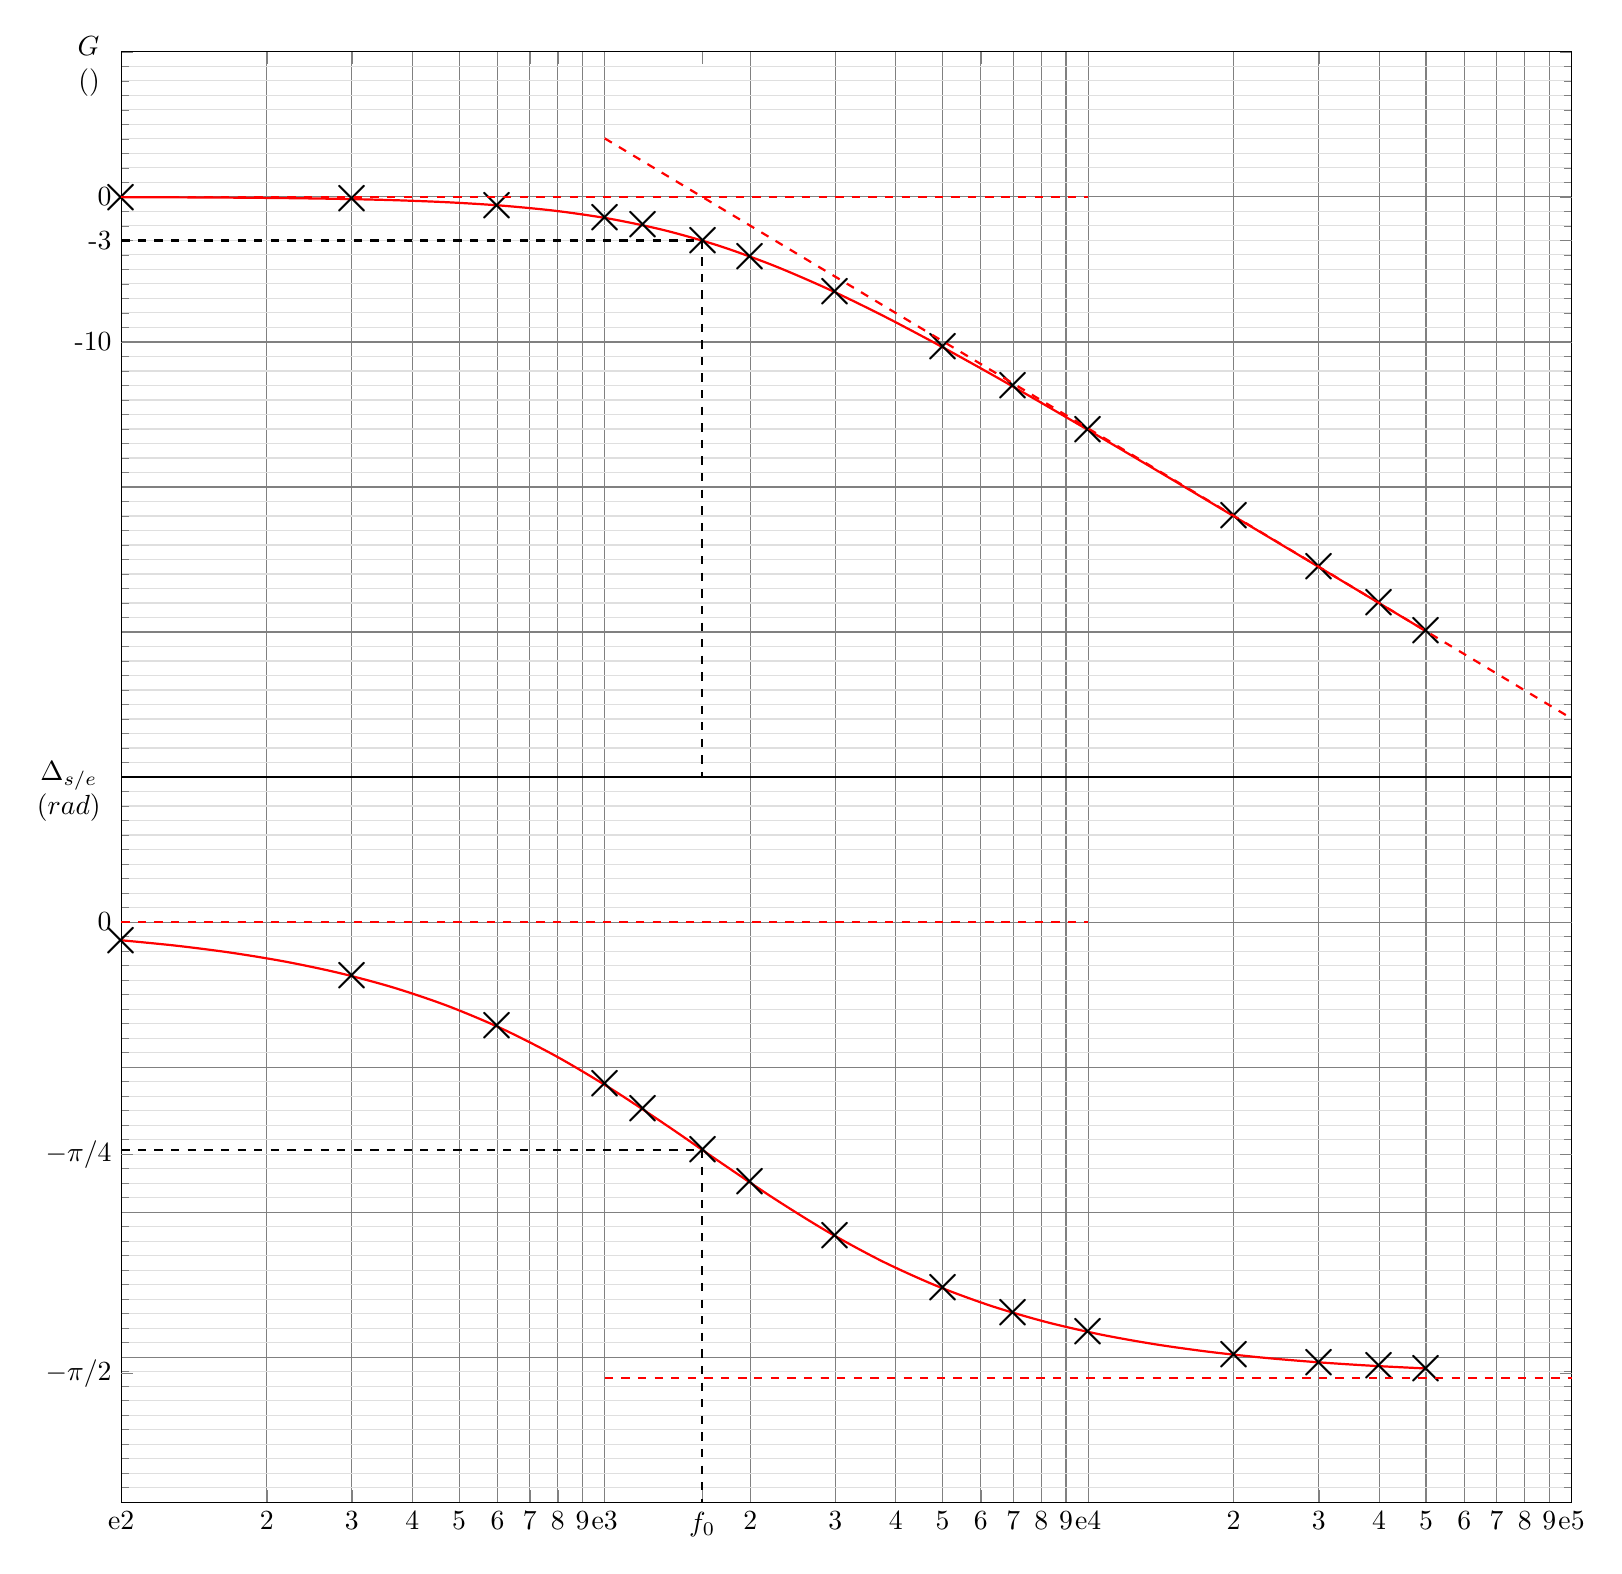
\begin{tikzpicture}
	\begin{semilogxaxis}[
			xmin=1e2, xmax=1e5,
			ymin=0, ymax=100,
			ytick={0, 10, ..., 100},
			yticklabels={},
			minor ytick={1, 2, ..., 99},
			extra y ticks={90, 87, 80, 40, 24, 8.9},
			extra y tick labels={0, -3, -10, 0, $-\pi/4$, $-\pi/2$},
			extra y tick style={grid=none},
			log ticks with fixed point,
			xtick={
					1e2, 2e2, 3e2, 4e2, 5e2, 6e2, 7e2, 8e2, 9e2,
					1e3, 2e3, 3e3, 4e3, 5e3, 6e3, 7e3, 8e3, 9e3,
					1e4, 2e4, 3e4, 4e4, 5e4, 6e4, 7e4, 8e4, 9e4,
					1e5},
			xticklabels={
					\num{e2}, 2, 3, 4, 5, 6, 7, 8, 9,
					\num{e3}, 2, 3, 4, 5, 6, 7, 8, 9,
					\num{e4}, 2, 3, 4, 5, 6, 7, 8, 9,
					\num{e5}},
			extra x ticks={\fop},
			extra x tick labels={$f_0$},
			extra x tick style={grid=none},
			width=20cm, height=20cm,
			grid=both,
			minor grid style={gray!25},
			major grid style={black!50},
			clip=false
		]
		% DIVIDE IN TWO
		\draw[thick]
		(axis cs:100,50) -- (axis cs:1e5,50);
		\node[anchor=east, align=center]
		at (axis cs:95,49) {$\Delta{\f_{s/e}}$\\$(\si{rad})$};
		\node[anchor=east, align=center]
		at (axis cs:95,99) {$G_{\dB}$\\$(\si{\dB})$};
		% GAIN
		\addplot[
			domain=1e2:5e4,
			smooth, thick, red]
		%{log10(\x)};
		{20*log10(1/sqrt(1+(\x/\fop)^2))+90}
		% node[scale=2, pos=0.0] {$\times$}
		% node[scale=2, pos=0.05] {$\times$}
		% node[scale=2, pos=0.1] {$\times$}
		% node[scale=2, pos=0.12] {$\times$}
		% node[scale=2, pos=0.145] {$\times$}
		% node[scale=2, pos=0.2] {$\times$}
		% node[scale=2, pos=0.3] {$\times$}
		% node[scale=2, pos=0.4] {$\times$}
		% node[scale=2, pos=0.5] {$\times$}
		% node[scale=2, pos=0.6] {$\times$}
		% node[scale=2, pos=0.8] {$\times$}
		% node[scale=2, pos=0.9] {$\times$}
		% node[scale=2, pos=1] {$\times$}
		;
		% \foreach \f in {1e2, 3e2, 6e2, 1e3, 1.2e3, 1.6e3, 2e3, 3e3, 5e3, 7e3, 1e4,
		% 		2e4, 3e4, 4e4, 5e4}{
		% 		\node[scale=2] at (axis cs:{\fpeval{\f}}, {20*log10(1/sqrt(1+(\fpeval{\f}/\fop)^2))+90}) {$\times$};
		% 		\node at (axis cs:{\fpeval{\f}},75) {\fpeval{\f}};
		% 		% \node[scale=2] at (axis cs:\fpeval{\f}, 75) {$\times$};
		% 	}
		\node[scale=2] at
		(axis cs:1e2,{20*log10(1/sqrt(1+(1e2/1.6e3)^2))+90}) {$\times$};
		\node[scale=2] at
		(axis cs:3e2,{20*log10(1/sqrt(1+(3e2/1.6e3)^2))+90}) {$\times$};
		\node[scale=2] at
		(axis cs:6e2,{20*log10(1/sqrt(1+(6e2/1.6e3)^2))+90}) {$\times$};
		\node[scale=2] at
		(axis cs:1e3,{20*log10(1/sqrt(1+(1e3/1.6e3)^2))+90}) {$\times$};
		\node[scale=2] at
		(axis cs:1.2e3,{20*log10(1/sqrt(1+(1.2e3/1.6e3)^2))+90}) {$\times$};
		\node[scale=2] at
		(axis cs:1.6e3,{20*log10(1/sqrt(1+(1.6e3/1.6e3)^2))+90}) {$\times$};
		\node[scale=2] at
		(axis cs:2e3,{20*log10(1/sqrt(1+(2e3/1.6e3)^2))+90}) {$\times$};
		\node[scale=2] at
		(axis cs:3e3,{20*log10(1/sqrt(1+(3e3/1.6e3)^2))+90}) {$\times$};
		\node[scale=2] at
		(axis cs:5e3,{20*log10(1/sqrt(1+(5e3/1.6e3)^2))+90}) {$\times$};
		\node[scale=2] at
		(axis cs:7e3,{20*log10(1/sqrt(1+(7e3/1.6e3)^2))+90}) {$\times$};
		\node[scale=2] at
		(axis cs:1e4,{20*log10(1/sqrt(1+(1e4/1.6e3)^2))+90}) {$\times$};
		\node[scale=2] at
		(axis cs:2e4,{20*log10(1/sqrt(1+(2e4/1.6e3)^2))+90}) {$\times$};
		\node[scale=2] at
		(axis cs:3e4,{20*log10(1/sqrt(1+(3e4/1.6e3)^2))+90}) {$\times$};
		\node[scale=2] at
		(axis cs:4e4,{20*log10(1/sqrt(1+(4e4/1.6e3)^2))+90}) {$\times$};
		\node[scale=2] at
		(axis cs:5e4,{20*log10(1/sqrt(1+(5e4/1.6e3)^2))+90}) {$\times$};
		\addplot[
			domain=1e2:1e4,
			smooth, red, dashed, thick]
		{0+90};
		\addplot[
			domain=1e3:1e5,
			smooth, red, dashed, thick]
		{-20*log10(\x/\fop)+90};
		\draw[dashed, thick]
		(axis cs:1e2,-3+90) -|
		(axis cs:\fop,50);
		% PHASE
		\addplot[
			domain=1e2:5e4,
			smooth, thick, red]
		{-20*atan(\x/\fop)*pi/180+40}
		% node[scale=2, pos=0.0] {$\times$}
		% node[scale=2, pos=0.05] {$\times$}
		% node[scale=2, pos=0.1] {$\times$}
		% node[scale=2, pos=0.12] {$\times$}
		% node[scale=2, pos=0.145] {$\times$}
		% node[scale=2, pos=0.2] {$\times$}
		% node[scale=2, pos=0.3] {$\times$}
		% node[scale=2, pos=0.4] {$\times$}
		% node[scale=2, pos=0.5] {$\times$}
		% node[scale=2, pos=0.6] {$\times$}
		% node[scale=2, pos=0.8] {$\times$}
		% node[scale=2, pos=0.9] {$\times$}
		% node[scale=2, pos=1] {$\times$}
		;
		\node[scale=2] at
		(axis cs:1e2,{-20*atan(1e2/1.6e3)*pi/180+40}) {$\times$};
		\node[scale=2] at
		(axis cs:3e2,{-20*atan(3e2/1.6e3)*pi/180+40}) {$\times$};
		\node[scale=2] at
		(axis cs:6e2,{-20*atan(6e2/1.6e3)*pi/180+40}) {$\times$};
		\node[scale=2] at
		(axis cs:1e3,{-20*atan(1e3/1.6e3)*pi/180+40}) {$\times$};
		\node[scale=2] at
		(axis cs:1.2e3,{-20*atan(1.2e3/1.6e3)*pi/180+40}) {$\times$};
		\node[scale=2] at
		(axis cs:1.6e3,{-20*atan(1.6e3/1.6e3)*pi/180+40}) {$\times$};
		\node[scale=2] at
		(axis cs:2e3,{-20*atan(2e3/1.6e3)*pi/180+40}) {$\times$};
		\node[scale=2] at
		(axis cs:3e3,{-20*atan(3e3/1.6e3)*pi/180+40}) {$\times$};
		\node[scale=2] at
		(axis cs:5e3,{-20*atan(5e3/1.6e3)*pi/180+40}) {$\times$};
		\node[scale=2] at
		(axis cs:7e3,{-20*atan(7e3/1.6e3)*pi/180+40}) {$\times$};
		\node[scale=2] at
		(axis cs:1e4,{-20*atan(1e4/1.6e3)*pi/180+40}) {$\times$};
		\node[scale=2] at
		(axis cs:2e4,{-20*atan(2e4/1.6e3)*pi/180+40}) {$\times$};
		\node[scale=2] at
		(axis cs:3e4,{-20*atan(3e4/1.6e3)*pi/180+40}) {$\times$};
		\node[scale=2] at
		(axis cs:4e4,{-20*atan(4e4/1.6e3)*pi/180+40}) {$\times$};
		\node[scale=2] at
		(axis cs:5e4,{-20*atan(5e4/1.6e3)*pi/180+40}) {$\times$};
		\addplot[
			domain=1e2:1e4,
			smooth, red, dashed, thick]
		{0+40};
		\addplot[
			domain=1e3:1e5,
			smooth, red, dashed, thick]
		{-20*pi/2+40};
		\draw[dashed, thick]
		(axis cs:1e2,-20*pi/4+40) -|
		(axis cs:\fop,0);
	\end{semilogxaxis}
\end{tikzpicture}
\end{document}
